\chapter{基于TreeCRF的高阶成分句法分析}
\label{cha:con-crf}

本章节提出了一个基于树形条件随机场的快速精准的神经成分句法分析器.
估计概率分布一直是自然语言处理领域的一个核心问题.
但是,在深度学习时代和前深度学习时代,不同于线性链条件随机场(linear chain CRF)在序列标注任务中的大量应用,由于Inside-Outside算法的高复杂度,还很少有工作将树形条件随机场应用到成分句法分析任务当中.
这里我们提出应用树形条件随机场到成分句法分析,核心的想法是批次化计算损失函数用到的Inside算法,使其能够支持在GPU上的大规模张量并行计算,与此同时结合基于高效自动求导机制的反向传播,避免了复杂的Outside算法的计算.
我们同样提出一个简单的两阶段解析方法,bracketing-then-labeling,来进一步提升分析器的效率.
为了提升解析的性能,受依存句法分析器的启发,我们引入了一个基于边界表示和仿射注意力的新打分方法,以及一个有效的Dropout策略.
在PTB、CTB5.1和CTB7上的实验表明我们的两阶段条件随机场分析器在使用和不使用BERT的两种设置上,达到了新的最佳性能,并且解析速度达到了1,000句每秒.

\section{引言}\label{sec:con-intro}

成分句法分析是自然语言处理领域一个基础但是富有挑战性的任务.
由于诸如宾州树库(Penn Treebank,PTB)、中文宾州树库(Penn Chinese Treebank,CTB)等大规模树库的标注,成分句法分析吸引了一大批研究者的关注.
同样的,句法分析输出的句法树也被证明对于大量的下游任务 \citep{akoury-etal-2019-syntactically,wang-etal-2018-tree}都有用.

作为最有影响力的工作之一,\cite{collins-1997-three}将概率上下文无关文法 (Probabilistic Context-Free Grammars,PCFGs)扩展到了词汇化文法(Lexicalized PCFGs).
由此开始,成分句法分析方法一直是这样的生成式模型(generative models)占据主导地位,并且其中广泛使用的Berkeley Parser采用了带隐式非终端结点标注的非词汇化概率上下文无关文法(Unlexicalized PCFGs) \citep{matsuzaki-etal-2005-probabilistic,petrov-klein-2007-improved}.
而在判别式方法(discriminative models),存在着两种主要方向.
第一种采取了以动态规划解码为基础的基于图的方法,训练时使用局部max-entropy估计 \citep{kaplan-etal-2004-speed}或者全局Max Margin方法 \citep{taskar-etal-2004-max}.
第二类则通过基于贪婪解码或者集束搜索(beam search)产生shift-reduce这样的转移序列来构建一棵树,这种方法被称为基于转移的方法 \citep{sagae-lavie-2005-classifier,zhu-etal-2013-fast}.

最近,得益于深度神经网络在上下文表示方面令人印象深刻的发展,成分句法分析取得了显著的进展.
其中,\cite{cross-huang-2016-span}的基于转移的分析器,以及\cite{stern-etal-2017-minimal}的基于图的分析器是两个具有代表性的工作.
作为判别式模型,两个分析器有很多的共同点,他们都使用了1)多层双向LSTM作为编码器;2)从双向LSTM的输出得到的minus feature作为区块的表示;3)利用MLP层来为区块打分;4)Max Margin的训练损失函数.
后续的大多数工作 \citep{gaddy-etal-2018-whats,kitaev-klein-2018-constituency}的主要设置都和这两个分析器一样, 并且都相比传统的非神经网络模型达到了更好的准确率,这特别是得益于由在大规模无标记文本上训练的语言模型输出的上下文词表示的使用 \citep{peters-etal-2018-deep,devlin-etal-2019-bert}.

然而尽管有这些显著的进展,现有的成分句法分析的研究仍然受两个相互关联的缺点困扰.
首先,解析速度(训练速度同理)很慢,并且很难满足现实系统的需要.
其次,显式的树/子树概率建模的缺失一定程度上影响来分析器输出的利用.
一方面,估计概率分布一直是自然语言处理领域的核心问题 \citep{le-zuidema-2014-inside}.
另一方面,与没有上下界的树的分值相比,树的概率可以作为一种软特征,更好的被更高层级的任务所利用 \citep{jin-etal-2020-relation},且子树的边缘概率可以支持更加复杂的最小贝叶斯风险解码 \citep{smith-smith-2007-probabilistic}.

事实上,\cite{finkel-etal-2008-efficient,durrett-klein-2015-neural}都通过建模树的条件概率$p(\boldsymbol{t}\mid\boldsymbol{x})$,提出了基于TreeCRF \citep{lafferty-etal-2001-crf}的成分句法分析器.
但是,由于损失函数和梯度计算需要的Inside-Outside算法的高复杂度(尤其是Outside算法),这些模型都极端低效.
而在深度学习时代,由于以前所有的工作都直接在CPU上运行Inside-Outside算法,而让模型频繁在CPU和GPU切换所需要的时间代价是昂贵的,因此效率问题变得更加严重.

本章节通过极大拓展\cite{stern-etal-2017-minimal}的基于图的分析器,提出了一个TreeCRF成分句法分析器.
主要的贡献在于我们为损失函数和梯度能够在GPU上能够直接计算,类似于章节\ref{cha:dep-crf},我们提出了Inside算法的批次化方法.
与此同时,我们发现Outside算法的可以通过自动的反向传播机制被高效的完成,使得Outside过程与Inside一样高效,这验证了\cite{eisner-2016-inside}出色的理论工作.
类似的,我们也批次化了CKY(Cocke–Kasami–Younger)算法,以支持高效的解码.

总体而言,我们在本章节做了如下的贡献.
\begin{itemize}
  \item 为了直接建模树和子树的概率,我们首次提出了一个快速精准的TreeCRF成分句法分析器.
        通过批次化技术支持Inside算法和CKY算法在GPU上的直接计算,长期以来一直困扰句法分析社区的效率问题在这里被很好的解决了.

  \item 我们提出了一个两阶段的解析方法bracketing-then-labeling:先产生无标记树骨干树(bracketing)再标注标签(labeling)的解析方法,这不仅更加高效,并且达到了比一阶段解析方法稍好的性能.

  \item 我们提出了基于区块表示的一个新的打分方法,以及基于仿射注意力机制的打分方法,比minus-feature方法表现的更好.
        我们同样表明,通过更好的模型及参数设置,比如Dropout,解析的性能可以被极大提升.

  \item 在中英文的三个基准数据集上的实验表明,我们提出的两阶段解析方法在使用BERT和不使用BERT \citep{devlin-etal-2019-bert}的两种设置下,在性能上都分别达到了新的最佳水准.
        在解析速度方面,我们的分析器可以达到大约1,000句每秒的解析速度.
\end{itemize}

\begin{figure}[tb]
  \centering
  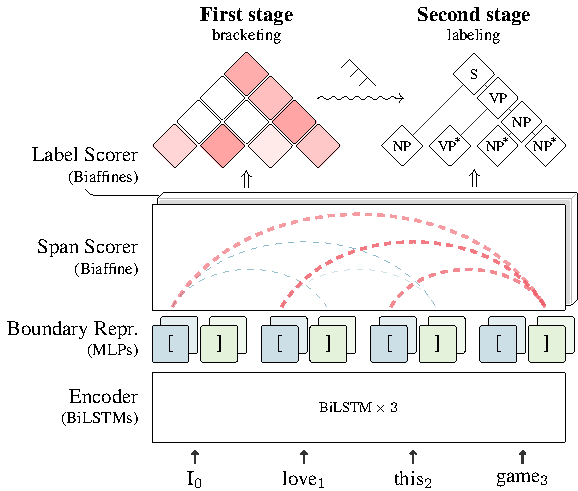
\includegraphics [scale=1.1]{figures/con-framework.pdf}
  \caption{模型架构.}
  \label{fig:con-framework}
\end{figure}

\section{两阶段TreeCRF解析}\label{sec:2stage-parsing}

如图~\ref{fig:con-tree-original}所示,对于一个由$n$个词组成的句子$\boldsymbol{x}=w_1,\dots,w_{n}$,一棵成分句法树$\boldsymbol{t}=\{((i, j),l)\mid 1\le i \le n,i \le j \le n,l \in \mathcal{L}\}$可以被分解为两个部分,即,$\boldsymbol{t}=(\boldsymbol{y}, \boldsymbol{l})$,其中$\boldsymbol{y}$是一棵无标签树(又称为bracketed tree),而$\boldsymbol{l}$是树中所有区块的标签按一定顺序产生的标签序列.
区块$(3,5,\texttt{VP})$可以等价表示为$\texttt{VP}_{3,5}$.

为了能够适应Inside算法和CKY算法,我们用NLTK工具包\footnote{\url{https://www.nltk.org}}将原始的树转换为了遵循乔姆斯基范式(Chomsky Normal Form,CNF)的二叉树形式,如图~\ref{fig:con-binaried-tree}所示.
特别地,连续的单链产生式被压缩为了一个标签,比如$\texttt{X}_{i,j} \rightarrow \texttt{Y}_{i,j}$会被压缩为一个$\texttt{X+Y}_{i,j}$.
根据前置实验,我们在二叉化原始树的时候,采用了左二叉.
在用CKY解码获得一棵最佳的树之后,CNF树会被恢复为原来的\textit{n}-ary形式.

\subsection{模型定义}\label{sub@sec:con-crf-model-definition}

在本章中,我们对成分句法分析采用了一个两阶段的解析框架bracketing-then-labeling.
这与传统的一阶段解析方法 \citep{stern-etal-2017-minimal,gaddy-etal-2018-whats}相比,不仅简化了模型架构,同样也提升了效率.

\noindent\textbf{第一阶段:bracketing.}
给定句子$\boldsymbol{x}$,第一阶段的目标是找到一个最优的无标签树$\boldsymbol{y}$.
一棵树的分值被分解为所有包含的区块(子树)的分值.
\begin{equation} \label{eq:tree-score}
  \mathrm{s}(\boldsymbol{x},\boldsymbol{y}) = \sum\limits_{(i,j)\in \boldsymbol{y}}\mathrm{s}(i,j)
\end{equation}

对于TreeCRF,条件概率为
\begin{equation}\label{eq:tree-prob}
  \begin{split}
    & p(\boldsymbol{y}\mid\boldsymbol{x})  = \frac{\exp({\mathrm{s}(\boldsymbol{x},\boldsymbol{y}))}}{Z(\boldsymbol{x}) \equiv \sum\limits_{\boldsymbol{y'} \in \mathcal{Y}(\boldsymbol{x})} {\exp({\mathrm{s}(\boldsymbol{x},\boldsymbol{y'}))}}}
  \end{split}
\end{equation}
其中$Z(\boldsymbol{x})$被称为partition term,$\mathcal{Y}(\boldsymbol{x})$是输入句子$\boldsymbol{x}$对应的所有合法句法树的集合.

给定所有的区块分值$\mathrm{s}(i,j)$,我们可以用CKY算法来找到一棵最优的无标签句法树$\boldsymbol{y}$.
\begin{equation} \label{eq:tree-argmax}
  \boldsymbol{y} = \arg\max_{\boldsymbol{y}^{\prime}} \mathrm{s}(\boldsymbol{x}, \boldsymbol{y}^{\prime}) = \arg\max_{\boldsymbol{y}^{\prime}} p(\boldsymbol{y}^{\prime} \mid \boldsymbol{x})
\end{equation}

\noindent\textbf{第二阶段:labeling.}
给定一个句子$\boldsymbol{x}$和一棵树$\boldsymbol{y}$,第二阶段独立地给每个区块$(i,j) \in \boldsymbol{y}$预测一个标签.
\begin{equation} \label{eq:label-argmax}
  l = \arg\max_{l^{\prime} \in \mathcal{L}} \mathrm{s}((i,j),l^{\prime})
\end{equation}
请注意训练时我们使用正确的无标签树来进行损失函数的计算.
对于一个长度为$n$的句子,所有的CNF树都包含同样$2n-1$多个的区块.
因此,这一阶段的时间复杂度为$O(n|\mathcal{L}|)$.

\noindent\textbf{时间复杂度分析.}
CKY的时间复杂度为$O(n^3)$.
因此,我们两阶段解析方法的总时间复杂度为$O(n^3+n|\mathcal{L}|)$.
相对应的,对于一阶段解析的CKY而言,算法需要为所有$n^2$个区块决定最优的标签,因此需要$O(n^3+n^2|\mathcal{L}|)$,其中$|\mathcal{L}|$通常来说都很大(比如对于表~\ref{table:con-statistics}中的英语来说为138).

\subsection{打分方法}

本章节引入了给区块和标签打分的模型架构,如图~\ref{fig:con-framework},大部分设置都遵循 \citep{stern-etal-2017-minimal},除了两个重要的修改:1)针对分值计算的边界表示和仿射注意力;2)和 \citep{dozat-etal-2017-biaffine}一样的更好的参数设置.

\noindent\textbf{模型输入.}
对于第$i$个词,其对应的输入向量$\mathbf{e}_i$是词向量和字级别表示的拼接:
\begin{equation} \label{eq:token-representation}
  \mathbf{e}_i = \mathbf{e}^{word}_i \oplus \mathrm{CharLSTM}(w_i)
\end{equation}
其中$\mathrm{CharLSTM}(w_i)$是将字序列输入到双向LSTM一样的输出向量 \citep{lample-etal-2016-neural}.
以前的工作表明将词性表示用$\mathrm{CharLSTM}(w_i)$代替会带来稳定的提升 \citep{kitaev-klein-2018-constituency}.
这同样简化了模型,因为不再需要额外预测词性.

\noindent\textbf{双向LSTM编码器.}
我们在输入向量上应用了三层双向LSTM以得到上下文表示.
我们分别用$\mathbf{f}_i$和$\mathbf{b}_i$来表示词$w_i$在顶层LSTM的前向和后向输出向量.

在这里,我们借用了大部分 \citep{dozat-etal-2017-biaffine}的依存句法分析器的参数设置(参考章节\ref{sec:dep-exps}).
我们发现其中的Dropout设置对于解析性能特别关键,这和原始的实现 \citep{stern-etal-2017-minimal}有两方面的不同.

首先,对于每个词$w_i$,$\mathbf{e}^{word}_i$和$\mathrm{CharLSTM}(w_i)$都作为一个整体被dropout,要么保持版本,要么称为$\mathbf{0}$向量.
如果其中一个向量被设置为了$\mathbf{0}$,则另一个会被乘以2倍作为补偿.
其次,相同LSTM层在不同的时间步(词)共享相同的dropout掩码 \citep{yarin-etal-2016-dropout}.

\noindent\textbf{边界表示.}
对于每个词$w_i$,我们参考 \citep{stern-etal-2017-minimal}的做法来组成上下文词向量\footnote{我们的前置实验表明$\mathbf{f}_i \oplus \mathbf{b}_{i+1}$相比于$\mathbf{f}_i \oplus \mathbf{b}_i$有稳定的提升. 可能的原因是$\mathbf{f}_i$和$\mathbf{b}_i$都使用$\mathbf{e}_i$作为输入,因此提供的信息冗余.}
\begin{equation}
  \mathbf{h}_i = \mathbf{f}_i \oplus \mathbf{b}_{i+1}
\end{equation}
$\mathbf{h}_i$的维度为800.

不同于直接应用一个单一的MLP层到$\mathbf{h}_i$上,我们发现一个词在一棵给定树的所有的区块中都必须作为其左边界或右边界.
因此,我们应用来两个MLP层来做这样的区分,并且分别获取左边界和右边界的表示向量.
\begin{equation}
  \label{mlp-boundaries}
  \mathbf{r}_i^{l}; \mathbf{r}_i^{r} =\mathrm{MLP}^{l} \left( \mathbf{h}_i \right); \mathrm{MLP}^{r} \left( \mathbf{h}_i \right)
\end{equation}
$\mathbf{r}_i^{l/r}$的维度$d$为500.
正如 \citep{dozat-etal-2017-biaffine}所指出的,MLP层缩减了$\mathbf{h}_i$的维度,并且更重要的是只保留了句法相关的信息,因此能够减轻过拟合的风险.

\noindent\textbf{仿射打分.}
给定边界表示,对于候选区块$(i,j)$,我们在左边界词$w_i$的表示和右边界词$w_j$的表示上利用仿射注意力为该区块打分.
\begin{equation} \label{eq:con-biaffine}
  \mathrm{s}(i,j) =  \left[
    \begin{array}{c}
      \mathbf{r}_{i}^{l} \\
      1
    \end{array}
    \right]^\mathrm{T}
  \mathbf{W} \mathbf{r}_{j}^{r}
\end{equation}
其中$\mathbf{W} \in \mathbb{R}^{d \times d}$.

计算区块标签的分值$\mathrm{s}((i,j),l)$时,需要在$\mathbf{h}_i$上应用额外两层MLP来获取相应的边界表示$\bar{\mathbf{r}}^{l/r}_i$(维度为$\bar{d}$).
接着我们使用$|\mathcal{L}|$个Biaffine($\mathbb{R}^{\bar{d} \times \bar{d}}$)来获取所有标签的分值.
由于$|\mathcal{L}|$非常大,我们对于$\bar{\mathbf{r}}^{l/r}_i$使用了稍小的维度$\bar{d}=100$(对于${\mathbf{r}}^{l/r}_i$则是500)以减轻内存和计算负担.

\noindent\textbf{前人打分方法.}
\citep{stern-etal-2017-minimal}对双向LSTM的输出使用了minus feature方法来得到区块的表示 \citep{wang-chang-2016-graph,cross-huang-2016-span},然后用MLP层得到区块的分值.
\begin{equation} \label{eq:minus-score}
  \mathrm{s}(i,j)=\mathrm{MLP}(\mathbf{h}_{i}-\mathbf{h}_{j})
\end{equation}
注意到 \citep{stern-etal-2017-minimal}等人的打分方法由于得到区块表示带来的高复杂度,难以应用到二阶区块结构上.
在实验部分我们表明我们的打分方法要明显更优越.

\subsection{训练损失函数}

对于一个训练的例子$(\boldsymbol{x},\boldsymbol{y},\boldsymbol{l})$,训练损失函数由两部分组成.
\begin{equation} \label{eq:final-loss}
  \mathit{L}(\boldsymbol{x}, \boldsymbol{y}, \boldsymbol{l}) = \mathit{L}^{bracket}(\boldsymbol{x}, \boldsymbol{y}) + \mathit{L}^{label}(\boldsymbol{x}, \boldsymbol{y}, \boldsymbol{l})
\end{equation}
第一项是句子级的全局TreeCRF损失,目的是最大化树的条件概率:
\begin{equation}\label{eq:bracket-loss}
  \begin{split}
    \mathit{L}^{bracket}(\boldsymbol{x},\boldsymbol{y})
    &= -\mathrm{s}(\boldsymbol{x}, \boldsymbol{y}) + \log Z(\boldsymbol{x})
  \end{split}
\end{equation}
其中$\log Z(\boldsymbol{x})$可以利用Inside算法在$O(n^3)$的时间复杂度内被计算.

第二项是在labeling阶段,区块级别的标准交叉熵损失函数.

\section{二阶TreeCRF}
\label{sec:con-2o-treecrf}

与章节~\ref{cha:dep-crf}类似,我们还进一步尝试了更加复杂的二阶子结构约束,在这个场景下,包含二阶子树的句法树分值被定义为
\begin{equation} \label{eq:2ostree-score}
  \mathrm{s}(\boldsymbol{x},\boldsymbol{y}) = \sum\limits_{(i,j)\in \boldsymbol{y}}\mathrm{s}(i,j)+\sum\limits_{(i,k,j)\in \boldsymbol{y}}\mathrm{s}(i,k,j)
\end{equation}
其中$(i,k,j)$这样的三元组是指$i \leq k < j$是区块$(i,j)$的分割点,并满足子区块$(i,k)$和$(k+1,j)$都在树中.

\subsection{基于Triaffine的二阶区块打分}
对于考虑分割点$k$的二阶区块$(i,k,j)$的打分,我们参考章节~\ref{cha:dep-crf},使用了一个Triaffine结构.
我们首先用三个额外的MLP层来进行和Biaffine类似的操作
\begin{equation}
  \label{con-mlp-sib}
  \mathbf{r}_i^{l'}; \mathbf{r}_i^{r'}; \mathbf{r}_i^{s} =\mathrm{MLP}^{l'/r'/s} \left( \mathbf{h}_i \right)
\end{equation}
$\mathbf{r}_i^{l'}; \mathbf{r}_i^{r'}; \mathbf{r}_i^{s}$是词$w_i$分别作为左边界、右边界和分割点对应的表示.
然后,我们对上述表示应用Triaffine结构
\begin{equation} \label{eq:con-triaffine}
  \mathrm{s}(i,k,j) =
  \left[
    \begin{array}{c}
      \mathbf{r}_{k}^{s} \\
      1
    \end{array}
    \right]^\mathrm{T}
  {\mathbf{r}_{i}^{l'}}^\mathrm{T}
  \mathbf{W}^\textit{triaffine}
  \left[
    \begin{array}{c}
      \mathbf{r}_{j}^{r'} \\
      1
    \end{array}
    \right]
\end{equation}
其中$\mathbf{W}^\textit{triaffine} \in \mathbb{R}^{d' \times d' \times d'}$是一个三维的张量.
我们设置$d'$的维度为100.

\begin{algorithm}[tb]
  \caption{批次化的Inside算法.}
  \begin{algorithmic}[1]
    \setlength{\commentindent}{.3\textwidth}
    \setlength{\algorithmicindent}{1.5em}
    \renewcommand{\algorithmiccomment}[1]{\unskip\hfill\makebox[\commentindent][l]{$\rhd$~#1}\par}
    \LetLtxMacro{\oldalgorithmic}{\algorithmic}
    \renewcommand{\algorithmic}[1][0]{%
      \oldalgorithmic[#1]%
      \renewcommand{\ALC@com}[1]{%
        \ifnum\pdfstrcmp{##1}{default}=0\else\algorithmiccomment{##1}\fi}%
    }
    %\begin{spacing}{1.2}
    % \begin{footnotesize}
    % \STATE $\forall 0 \le i \le n ~ C_{i, i} = 0$
    % \COMMENT $\rhd$ initialization
    \STATE \textbf{define:} $S \in \mathbb{R}^{n \times n \times B}$ \COMMENT{$B$ is \#sents in a batch}
    % \STATE \hspace{\algorithmicindent}
    % \STATE \textbf{Output:} $ C_{0, n} = \log Z(\boldsymbol{x})$
    %   \COMMENT{balabala}

    \STATE \textbf{initialize:} all $S_{:, :} = 0$
    % \STATE $S_{i, i+1} = s_{i, i+1}$ \COMMENT{$w$ is 1}
    \FOR [span width]{$w = 1$ \TO $n$}
    \STATE \emph{Parallel computation on $0 \le i$,$j<n$,$~r$,$0\le b<B$}
    \STATE $S_{i, j=i+w} = \log \sum\limits_{i \le r < j} \exp \left( S_{i, r}+S_{r+1, j} \right)  + s(i, j) $ \label{line:sum-product}\\
    %\textbf{batchify:} $0 \le i$; $j=i+w < n$
    \ENDFOR
    \RETURN $S_{0, n-1} \equiv \log Z(\boldsymbol{x})$
    % \end{footnotesize}
    %\end{spacing}
  \end{algorithmic}
  \label{alg:inside}
\end{algorithm}


下面我们描述如何通过批次化Inside算法和CKY算法以支持在GPU上的直接计算,来进行高效的训练和解码.
我们同样表明对于成分句法分析,复杂的Outside算法可以被自动求导机制支持的反向传播完成.

\subsection{高效的TreeCRF计算方法}

对于TreeCRF的损失函数(公式~\ref{eq:bracket-loss})里的配分项$Z(\boldsymbol{x})$和特征梯度,所有以前在TreeCRF解析上的工作 \citep{finkel-etal-2008-efficient,durrett-klein-2015-neural}都是通过显式地在CPU上进行了Inside-Outside算法计算得到的.
不同于线性链CRF,树状结构的CRF的批次化看起来要复杂很多.

在这里,我们发现实现一个批次化的Inside算法是可行的,如算法~\ref{alg:inside}所示.
关键的想法是将一个批次的所有实例中宽度相同的区块分值打包到一个大的张量中.
这使得我们可以通过高效的大规模张量操作进行计算和合并.
由于对所有的$0 \le i$,$j<n$,$~r$,$0\le b<B$而言,在GPU上的计算都是并行的,因此算法仅需要$O(n)$步.
我们的代码会给出更多的技术细节.

\subsection{基于反向传播的Outside算法的替代}

传统上,Outside算法被认为对于子树边缘概率和特征梯度的计算是不可或缺的.
事实上,Outside算法通常至少要两倍慢于Inside算法.
而Outside算法的批次化也要复杂的多.
幸运的是,这个问题在深度学习时代被很好的解决了,基于自动求导机制支持的反向传播可以方便的获取梯度.
\citet{eisner-2016-inside}提出了理论上的等价性证明.
由于我们在前向过程使用来批次化的Inside算法,因此反向传播过程也是通过大规模张量并行计算的,可以视为同样高效.

值得注意的是通过用区块分值$\mathrm{s}(i,j)$对$\log Z(\boldsymbol{x})$求偏导(同样由自动的反向传播完成),我们可以自然的得到区块$(i,j)$的边缘概率,也就是梯度.
\begin{equation} \label{eq:con-partial-derivative}
  p((i, j)\mid\boldsymbol{x}) = \frac{\partial \log Z(\boldsymbol{x})}{\partial \mathrm{s}(i, j)}
\end{equation}
边缘概率在很多下游任务都可以作为一种很有用的软特征.
更多细节可以参考\citet{eisner-2016-inside}.

\subsection{解码}

正如上面提到的,解析过程中,我们应用CKY算法来获取一棵最佳的句法树,如公式~\ref{eq:tree-argmax}所示.
和Eisner算法一样,CKY算法和成分句法分析的Inside算法几乎一样,除了其中的sum-product被替换为了max-product(参考算法~\ref{alg:inside}的行~\ref{line:sum-product}),因此可以被同样高效的批次化.
为了进行MBR解码,我们直接将区块分值$\mathrm{s}(i,j)$换成式~\ref{eq:tree-score}和式~\ref{eq:tree-argmax}的边缘概率$p((i,j)\mid\boldsymbol{x})$.
然而,我们发现这在成分句法上带来了很微弱的提升.

\section{实验}
\label{sec:con-experiments}

\noindent\textbf{参数设置.}
我们直接采用\citet{dozat-etal-2017-biaffine}的依存句法分析器里面的大部分参数设置,没有进一步的改动.
唯一的区别是我们用了CharLSTM词表示,而非词性embedding.
CharLSTM里自向量、词向量以及CharLSTM输出向量的维度分别为50、100和100.
所有Dropout的比率为0.33.
一个批次数据的大小约为5,000个词.
训练过程持续至多不超过1,000次迭代,并且如果Dev数据上的最高结果连续100次不提示,那么训练就会提前停止.

\begin{table*}[tb!]
    % \setlength{\tabcolsep}{8.6pt}
    \centering
    \begin{tabularx}{\textwidth}{lccccccccc}
        \toprule
                                   & \multicolumn{3}{c}{PTB} & \multicolumn{3}{c}{CTB5.1} & \multicolumn{3}{c}{CTB7}                                                                                                       \\
        % \cmidrule(lr){2-4}\cmidrule(lr){6-8}\cmidrule(lr){10-12}
                                   & P                       & R                          & F                        & P              & R              & F              & P              & R              & F              \\
        \midrule
        % \\[-8pt]
        Max Margin (one-stage)     & 93.70                   & 93.73                      & 93.72                    & 90.60          & 90.48          & 90.54          & 86.85          & 86.08          & 86.47          \\
        \textsc{Crf} (one-stage)   & 93.44                   & 93.75                      & 93.60                    & 91.08          & 90.98          & 91.03          & 87.10          & 86.75          & 86.93          \\[3pt]
        \textsc{Crf} (two-stage)   & 93.77                   & 93.96                      & 93.86                    & 90.91          & 91.09          & 91.00          & 87.27          & 87.00          & 87.13          \\
        \qquad w/o MBR             & 93.75                   & 93.85                      & 93.80                    & \textbf{90.93} & 91.10          & 91.02          & 87.21          & 86.89          & 87.05          \\
        % \hline
        \qquad minus feature       & 93.40                   & 93.35                      & 93.37                    & 90.60          & 90.51          & 90.56          & 86.96          & 86.24          & 86.60          \\
        \qquad vanilla dropout     & 92.80                   & 93.00                      & 92.90                    & 89.68          & 89.68          & 89.68          & 85.55          & 85.54          & 85.54          \\
        \textsc{Crf2o} (two-stage) & \textbf{93.87}          & \textbf{93.98}             & \textbf{93.93}           & 90.86          & \textbf{91.24} & \textbf{91.05} & \textbf{87.34} & \textbf{87.16} & \textbf{87.25} \\

        \bottomrule
    \end{tabularx}
    \caption{Dev数据上的结果. 所有模型都使用了随机初始化的词向量.}
    \label{table:con-dev}
\end{table*}

\subsection{模型比较}

我们在Dev数据上从两方面对模型进行深入探究:1)TreeCRF与Max Margin训练损失函数的对比;2)两阶段解析和一阶段解析的对比.
表~\ref{table:con-dev}的前三行显示了相应的结果.
这三个模型使用了相同的打分方法和参数设置.
参考前人的经验 \citep{stern-etal-2017-minimal},一阶段解析的模型只用带标签的区块$\mathrm{s}((i,j),l)$的分值.
为了验证两阶段解析的有效性,我们同样列出了``\textsc{Crf} (one-stage)''的结果,``\textsc{Crf} (one-stage)''是指直接在有标签区块上打分.
\begin{equation} \label{eq:tree-label-score}
  \mathrm{s}(\boldsymbol{x},\boldsymbol{y},\boldsymbol{l}) =
  \sum_{(i,j),l \in (\boldsymbol{y}, \boldsymbol{l})} \mathrm{s}((i,j),l)
\end{equation}
如章节\ref{sub@sec:con-crf-model-definition}的最后一段所讨论的,一阶段解析的Inside算法和CKY算法相比于两阶段解析要复杂一点.

从表格的前两行我们可以看到,在一阶段解析的框架下,TreeCRF损失函数在英语上带来了相似的结果,但是在中文数据集上稳定超过Max Margin方法0.5的$\mathrm{F}_1$值.
Max Margin方法由额外的超参数,即margin值,该值根据在英语上调整的结果为1,并且为了方便没有在中文上进一步调整.
我们猜测Max Margin方法在中文数据上的结果如果进一步调参的话可能还会有提升.
总体上,我们可以认为两种训练损失函数达到了非常相近的结果,但是TreeCRF方法有额外的概率建模的优势.

如果对表中第二行和第三行的结果进行比较,两种TreeCRF解析器在CTB5.1上的结果十分相近,而两阶段解析的解析器在PTB和CTB7上相比于一阶段解析的方法超过了大约0.2的$\mathrm{F}_1$值.
因此我们可以认为我们提出的两阶段解析在简单性和效率上要好于一阶段解析(参考表~\ref{table:speed}),并且没有损失性能.

最后,我们比较了同样的两阶段解析设置下的一阶\textsc{Crf}模型和二阶\textsc{Crf2o}的模型的结果.
与一阶模型相比,二阶模型在PTB上的结果几乎与一阶模型一样,这可能是由于英语数据的基线结果已经很好了.
二阶模型在CTB5.1和CTB7上分别有0.3和0.4的提升,表明引入二阶结果对于成分句法分析仍然有一定的作用.

\subsection{消融实验}

为了了解我们提出的框架中每个单独的模块所发挥的作用,我们在一阶模型上,通过每次去除一个模块,在Dev数据上进行了消融实验.
结果见表~\ref{table:con-dev}的最后四行.

\noindent\textbf{MBR解码的影响.}
我们默认在边缘概率上使用CKY解码.
行``w/o MBR''给出了在区块分值上解码的结果.
由于通常认为MBR解码在理论上要优于原始的解码方式,这样的比较给出了一些有趣的视角.
但是,从结果中可以明显的看到两种解码方式的结果近乎一样.

\noindent\textbf{打分方法的影响.}
为了衡量我们提出的新的打分方法带来的影响,我们将仿射打分器恢复到了原来 \citep{stern-etal-2017-minimal}(参考公式~\ref{eq:minus-score})采用的``minus feature''方法.
可以清晰的看到我们提出的打分方法要优于广泛使用的minus-feature方法,并且在所有三个数据上有大约0.5$\mathrm{F}_1$值的显著一致的提升.

\noindent\textbf{Dropout策略的影响.}
我们保持其他模型设置都不变,然后将我们参考自 \citep{dozat-etal-2017-biaffine}的Dropout策略换成 \citep{stern-etal-2017-minimal}采用的原始Dropout方式.
这导致了三个数据集上结果的显著下降,分别是0.96、1.39和1.59$\mathrm{F}_1$值的下降.
\citep{kitaev-klein-2018-constituency}用一个自注意力编码器替换了 \citep{stern-etal-2017-minimal}的双向LSTM编码器,通过分离上下文和位置注意力,达到了1.0 $\mathrm{F}_1$值的巨大提升.
类似地,这里我们表明基于双向LSTM编码器的解析器,如果有合适的参数设置,那么和自注意力编码器相比仍然很有竞争力.

\noindent\textbf{二阶特征的影响.}
表个最后一行列出了引入二阶特征的模型\textsc{Crf2o}的结果.
除了引入了考虑分割点的二阶分值,\textsc{Crf2o}和一阶模型\textsc{Crf}完全一样,都采用了两阶段解析,一致的编码器和打分方法.
可以看到在三个数据集上,\textsc{Crf2o}取得了最高的结果,但是提升并不显著.
在三个数据集上的提升分别是0.07、0.05和0.12.
这显示引入二阶特征的作用十分微弱.

\begin{table}[tb!]
	% \setlength{\tabcolsep}{15pt}
	\centering
	\caption{PTB的Test数据上的解析速度比较.}
	\begin{tabular}{lcr}
		\toprule
		                                                      & F$_1$                    & Sents/sec     \\
		\midrule
		% \\[-8pt]
		\citet{petrov-klein-2007-improved}  (Berkeley Parser) & 90.1\textcolor{white}{0} & 6             \\
		\citet{zhu-etal-2013-fast} (ZPar)                     & 90.4\textcolor{white}{0} & 90            \\
		\citet{stern-etal-2017-minimal}                       & 91.79                    & 76            \\
		\citet{shen-etal-2018-straight}                       & 91.8\textcolor{white}{0} & 111           \\
		\citet{kitaev-klein-2018-constituency}                & 93.55                    & 332           \\
		\citet{gomez-rodriguez-vilares-2018-constituent}      & 90.0\textcolor{white}{0} & 780           \\[3pt]
		\textsc{Crf} (one-stage)                              & 93.71                    & 990           \\
		\textsc{Crf2o} (two-stage)                            & \textbf{94.22}           & 598           \\
		\textsc{Crf} (two-stage) w/ MBR                       & 94.12                    & 743           \\
		\textsc{Crf} (two-stage) w/o MBR                      & 94.08                    & \textbf{1092} \\
		
		
		\bottomrule
	\end{tabular}
	\label{table:speed}
\end{table}

\subsection{速度比较}
表格~\ref{table:speed}列出了不同的解析器关于解析速度方面的比较.
公平比较的需要,我们的模型都运行在Intel Xeon E5-2650 v4 CPU和Nvidia GeForce GTX 1080 Ti GPU.
Berkeley Parser和ZPar是两个最具代表性的非神经网络的解析器,并且没法利用GPU.
\citep{stern-etal-2017-minimal}应用了Max Margin方法训练并且在CPU上进行了类CKY的解码.
\citep{kitaev-klein-2018-constituency}使用了自注意力编码器,并用Cython做了加速.

可以看到我们的一阶段TreeCRF解析器由于直接在GPU上解码,因此比前人的解析器要快得多.
在一阶模型上,我们的两阶段解析器每秒可以解析1,092句,是 \citep{kitaev-klein-2018-constituency}的三倍快.
当然,值得注意的是如果采用了我们提出的批次化技术, \citep{stern-etal-2017-minimal,kitaev-klein-2018-constituency}的方法可能和我们的一样快.

\citep{gomez-rodriguez-vilares-2018-constituent}的解析器将句法分析任务视为一个序列标注问题,因此同样十分高效.
但是他们的结果还很差,如表~\ref{table:con-test}所示.

两阶段解析器相比于一阶段解析器要快大约10\%.
相比于我们之前讨论的时间复杂度差异(参考章节~\ref{sub@sec:con-crf-model-definition}),这个差距显得似乎不是特别明显.
一个利用是这两种解析器都共享了相同的编码和打分组块,这可能占用了解析的大部分时间.

使用MBR解码额外需要运行一次Inside算法和反向传播来计算边缘概率,因此相对来说效率要差一些.
如表~\ref{table:con-dev}所示,在有和没有MBR解码的两个设置下,结果的差异很小.

在使用MBR解码和不使用MBR解码两种场景下,一阶模型都分别比二阶模型快了大约200句每秒,但是却达到了相似都性能(见表~\ref{table:con-test}).

\begin{table*}[tb]
    \centering
    \caption{Test数据的结果.}
    \begin{tabularx}{\textwidth}{lccccccccc}
        \toprule
                                                        & \multicolumn{3}{c}{PTB}  & \multicolumn{3}{c}{CTB5.1} & \multicolumn{3}{c}{CTB7}                                                                                                                                     \\
                                                        & P                        & R                          & F                        & P                        & R                        & F                        & P              & R              & F              \\
        \midrule
        % \\[-8pt]
        % \multicolumn{4}{l}{\textbf{Random word embeddings}} \\
        % \cite{liu-zhang-2017-shift}                     &         92.1\textcolor{white}{0}   &         91.3\textcolor{white}{0}   &         91.7\textcolor{white}{0}   &&         85.9\textcolor{white}{0}   &         85.2\textcolor{white}{0}   &         85.5\textcolor{white}{0}   &&         -      & -              & -              \\
        \cite{stern-etal-2017-minimal}                  & 92.98                    & 90.63                      & 91.79                    & -                        & -                        & -                        & -              & -              & -              \\
        % \cite{liu-2018-improving}                       &         -      &         -      &         91.2   &&         -      &         -      &         84.1   &&         -      & -              & -              \\
        % \cite{fried-klein-2018-policy}                       &         -      &         -      &         92.2   &&         -      &         -      &         87.0   &&         -      & -              & -              \\
        % \cite{stern-etal-2017-effective}                &         92.57   &          92.56   &         92.56  \\
        \cite{gaddy-etal-2018-whats}                    & 92.41                    & 91.76                      & 92.08                    & -                        & -                        & -                        & -              & -              & -              \\
        \cite{kitaev-klein-2018-constituency}           & 93.90                    & 93.20                      & 93.55                    & 88.09                    & 86.78                    & 87.43                    & -              & -              & -              \\
        \cite{gomez-rodriguez-vilares-2018-constituent} & -                        & -                          & 90.0\textcolor{white}{0} & -                        & -                        & 84.4\textcolor{white}{0} & -              & -              & -              \\
        \cite{shen-etal-2018-straight}                  & 92.0\textcolor{white}{0} & 91.7\textcolor{white}{0}   & 91.8\textcolor{white}{0} & 86.6\textcolor{white}{0} & 86.4\textcolor{white}{0} & 86.5\textcolor{white}{0} & -              & -              & -              \\
        \cite{teng-zhang-2018-two} %(w/ pretrained)
                                                        & 92.5\textcolor{white}{0} & 92.2\textcolor{white}{0}   & 92.4\textcolor{white}{0} & 87.5\textcolor{white}{0} & 87.1\textcolor{white}{0} & 87.3\textcolor{white}{0} & -              & -              & -              \\

        \cite{vilares-etal-2019-better}                 & -                        & -                          & 90.60                    & -                        & -                        & 85.61                    & -              & -              & -              \\
        \cite{zhou-zhao-2019-head} w/ pretrained        & 93.92                    & 93.64                      & 93.78                    & 89.70                    & 89.09                    & 89.40                    & -              & -              & -              \\[3pt]
        \textsc{Crf}                                    & 93.84                    & 93.58                      & 93.71                    & 89.18                    & 89.03                    & 89.10                    & 87.66          & 87.21          & 87.43          \\
        \textsc{Crf2o}                                  & 94.06                    & 93.84                      & 93.95                    & 89.04                    & 88.68                    & 88.86                    & 87.86          & 87.40          & 87.63          \\
        \textsc{Crf} w/ pretrained                      & 94.23                    & 94.02                      & 94.12                    & 89.71                    & \textbf{89.89}           & \textbf{89.80}           & 88.84          & 88.36          & 88.60          \\
        \textsc{Crf2o} w/ pretrained                    & \textbf{94.29}           & \textbf{94.15}             & \textbf{94.22}           & \textbf{89.97}           & 89.47                    & 89.72                    & \textbf{88.95} & \textbf{88.56} & \textbf{88.76} \\[1pt]
        \midrule
        \\[-20pt]
        \cite{kitaev-klein-2018-constituency} w/ ELMo   & 95.40                    & 94.85                      & 95.13                    & -                        & -                        & -                        & -              & -              & -              \\
        \cite{kitaev-etal-2019-multilingual} w/ BERT    & 95.73                    & 95.46                      & 95.59                    & 91.96                    & 91.55                    & 91.75                    & -              & -              & -              \\[3pt]
        \textsc{Crf} w/ BERT                            & \textbf{95.85}           & \textbf{95.53}             & \textbf{95.69}           & 92.51                    & 92.04                    & 92.27                    & 91.73          & \textbf{91.38} & 91.55          \\
        \textsc{Crf2o} w/ BERT                          & 95.73                    & 95.45                      & 95.59                    & \textbf{92.75}           & \textbf{92.18}           & \textbf{92.47}           & \textbf{91.93} & 91.31          & \textbf{91.62} \\
        \bottomrule
    \end{tabularx}
    \label{table:con-test}
\end{table*}



\subsection{主要结果}
表~\ref{table:con-test}显示了有和没有ELMo/BERT这两种设置下,Test数据集上的主要最终结果.

除了\citet{zhou-zhao-2019-head},大部分前人的结果都没有使用预训练的词向量,而是用了随机初始化的版本.
他们在英文上使用了Glove词向量,中文上用了structured skip-gram词向量.
对于预训练词向量,我们在英文PTB上用了100维的Glove\footnote{\url{https://nlp.stanford.edu/projects/glove}},中文上采用了\citet{li-etal-2019-attentive}的设置,使用基于Gigaword 3rd Edition训练的词向量,我们同样尝试了\citet{zhou-zhao-2019-head}分享的structured skip-gram词向量,最终的结果和前者差不多.
可以明显看到我们的解析器极大受益于预训练词向量的使用.

我们同样与最近的一些成分句法分析相关工作做了对比.
可以看到我们的基于双向LSTM编码器的解析器极大的超越了基本的\citet{stern-etal-2017-minimal},这大部分要归功于新的打分方法,以及Dropout之类的参数设置.
和在Dev数据上的趋势一致,我们的二阶模型\textsc{Crf2o}和一阶模型\textsc{Crf}的结果近乎一致,其中\textsc{Crf2o}在PTB和CTB7上的结果超越了\textsc{Crf},在CTB51上要次于\textsc{Crf},但是差异都不大.
与之前最佳的自注意力解析器相比\citet{kitaev-klein-2018-constituency},我们的一阶解析器分别在英文PTB和中文CTB5.1有0.16以及1.67的绝对提升,并且不包含任何语言特定的实验设置.

\citet{zhou-zhao-2019-head}的CTB5.1结果得自重新运行他们开源的代码,使用了预测的词性.
我们参考了他们描述\footnote{\url{https://github.com/DoodleJZ/HPSG-Neural-Parser}}来产生预测词性.
值得注意的是他们的汇报的CTB5.1结果意外使用了正确的词性.
我们用正确词性重新跑了他们的代码,在CTB5的Test数据的结果是92.14,与他们论文汇报的结果十分接近.
我们的解析器使用正确词性之后的结果达到了92.66的$\mathrm{F}_1$值.
关于他们论文的另一个细节需要澄清:对于中文上的依存句法分析,他们使用了两种不同的数据分割设置,并且都用了Stanford Dependencies 3.3.0以及正确词性.

表格的最后三行列出了在使用ELMo/BERT设置下的结果.
对于PTB,我们参考\citet{kitaev-etal-2019-multilingual},使用了\texttt{bert-large-cased}\footnote{\url{https://github.com/huggingface/transformers}}(24 layers,1024 dimensions,16 heads),对于CTB则使用了\texttt{bert-base-chinese}(12 layers,768 dimensions,12 heads).
可以明显看到无论是在一阶\textsc{Crf}模型和二阶\textsc{Crf2o}模型上,使用BERT表示都可以极大帮助性能的提升,最终两种解析器的结果趋于一致.
我们的解析器同样超过了\citet{kitaev-etal-2019-multilingual}的多语言解析器,这里他们用了额外了多语言资源.
总体而言,我们的解析器在两个语言和不同的设置下都达到了当前最佳的结果.

\section{本章小结}\label{sec:con-conclusions}

本章中,我们提出了一个快速精准的神经TreeCRF成分句法分析器.
我们表明Inside算法和CKY算法可以被高效的批次化,以支持在GPU上的大规模张量并行计算,进而带来显著的效率提升.
基于自动求导机制的反向传播和Inside算法一样高效,并且取代了Outside算法来进行梯度的计算.
在中英文三个基准数据集上的实验展现了很多富有前景的发现.
第一,简单的两阶段bracketing-then-labeling解析方法比一阶段解析更加高效,并且没有损害解析器的性能.
第二,我们新提出的打分方法相比于前人的基于minus feature的方法达到了更高的结果.
第三,我们引入的一些诸如Dropout的参数设置可以极大提升解析的性能.
最后,我们提出的解析器达到了新的最佳结果,并且可以解析超过1,000句每秒.
